\ofsubsection{Gold Saucer}
%
\ofquote{"Bem vindo a Gold Saucer! Você será comovido e empolgado, emocionado e aterrorizado! Levado de uma emoção a outra como nunca experienciou! Crie suas memórias hoje."}{Comercial}
%
\begin{center} \includegraphics[width=\columnwidth]{./art/goldsaucer/goldsaucer.jpg} \end{center}
%
\vfill
%
\accf{Gold Saucer} é um parque de diversões com uma enorme variedade de jogos e atrações para os jogadores aproveitar e participarem. 
Assim sendo, o conteúdo a seguir é, em sua maioria, uma lista de atrações do parque e suas respectivas regras.
Gold Saucer é construído como uma alta torre, rodeada por várias estruturas grandes que contém diferentes atrações.
A entrada do parque só pode ser alcançada através de um teleférico, o passe de entrada é de 50G por pessoa, já incluída a tarifa.
Há também, a opção vitalícia de 500G. Além disso, entrar numa atração normalmente custa Pontos de Ouro (PO), que são as únicas moedas aceitas dentro do parque.
Elas podem ser compradas ou vendidas na entrada ao custo de 1 PO por 50G.
logo após a entrada, os jogadores estarão no eixo central, de onde podem se locomover entre os principais locais do parque através de uma série de tubos.
%
\vfill
%
\begin{center} \includegraphics[width=\columnwidth]{./art/goldsaucer/hauntedhouse.jpg} \end{center}
%
\newpage
%
Este documento foca nas atrações principais do parque e oferece regras detalhadas de como as recriar em seu jogo.
Por outro lado, há também muitas atrações menores em Gold Saucer, algumas das quais estão listadas abaixo:\ofrow
\ofbullet{\accf{Cartomante:} um ser estranho que parece com um grande brinquedo de pelúcia com um gato em cima. Ele oferece leitura da sorte ao grupo pelo custo de 2 GP, um serviço que eles só podem usar uma vez. O MJ deve garantir que o cartomante dê ao grupo uma predição precisa ou conselho útel para o futuro.}
\ofbullet{\accf{Gôndola:} pelo preço de 1 GP por pessoa, o grupo pode andar na grande gôndola, que os permite ter uma bela visão de todo o parque de seu ponto mais alto. Se eles entrarem nela à meia noite, também podem observar os fogos de artifícios diários de Gold Saucer. O local perfeito para um encontro!}
\ofbullet{\accf{Casa Assombrada:} um castelo arrepiante que foi preparado para assustar seus visitantes através de adereços falsos, como fantasmas, esqueletos e aranhas espalhadas. Ao entrar pela primeira vez, cada jogador têm de realizar um teste de DF~8 ou ficar assustado ou apavorado. A casa assombrada funciona como um hotel, o grupo pode passar a noite aqui pelo preço de 1 GP por pessoa.}
%
\\\\
%
\ofquote{"Enquanto o carrinho faz ZOOM, você faz BANG BANG, então tem PHEW PHEW e você os destrói com um grande BOOM. Bem simples, né?"\\}{Funcionário}
%
%
%
%
%
%
\begin{center} \includegraphics[width=\columnwidth]{./art/goldsaucer/shootingcoaster.jpg} \end{center}
A \accf{Montanha-russa atiradora} é um jogo de montanhas-russas cuja entrada custa 1 GP por pessoa. 
Cada assento tem uma torreta acoplada que os visitantes podem usar para disparar contra várias projeções que surgem ao longo do trajeto.
Acertar um objeto projetado fornece aos jogadores uma quantidade de pontos que se revertem em prêmios ao se conseguir altas pontuações.
A duração do trajeto é separado em 5 rodadas.
No começo de cada um deles, o MJ rola uma quantidade de dados igual ao tamanho do grupo mais 1, a fim de determinar quais projeções aparecem nessa rodada.
Durante cada rodada, cada jogador tem seu turno, no qual podem atirar em uma das projeções à sua escolha.
Para fazer isso, eles devem passar num teste, a DF depende do tipo de projeção, pois algumas são rápidas e menores, e por isso, mais difíceis de atingir.
No entanto, aquelas que são mais difíceis de acertar também dão mais pontos.
Os personagens que puderem usar Arcos ou Armas de fogo, ou têm outras experiências com armas à distância, têm vantagem nesse teste.
As projeções desaparecem se forem atingidas ou ao final da rodada.
A tabela abaixo mostra todas aquelas possíveis, a quantidade de dados (Qd.) em que aparecem. A DF necessária para os acertar e quantos pontos fornecem.
%
\\\\
%
\oftable{p{0.2\columnwidth} p{0.3\columnwidth} p{0.2\columnwidth} r}
{\accf{Qd.} & \accf{Nome} & \accf{DF} & \accf{Pontos}}
{
	1 & Cacto 	& 5  & 10 \ofrow
	2 & Balão & 6  & 15 \ofrow		
	3 & Avião   & 7  & 20 \ofrow
	4 & Fantasma 	& 8  & 30 \ofrow
	5 & Estrela 	& 9  & 50 \ofrow
	6 & OVNI   	& 10 & 70 \ofrow			
}
%
\\\\
%
Durante o passeio, cada jogador deve anotar a quantidade de pontos que conseguiu e depois da 5º rodada ter terminado, cada um deles recebe os seguintes prêmios baseados em sua pontuação.
%
\\\\
%
\oftable{p{0.5\columnwidth} p{0.5\columnwidth}}
{\accf{Pontuação} & \accf{Prêmio}}
{
	Menor que 25 & Poção \ofrow
	de 25 a 50 & DEF+ \ofrow
	de 50 a 75 & Super poção \ofrow		
	de 75 a 100 & Amuleto Moogle\ofrow
	Maior que 100 & Fita de cabelo  																				
}
%
\\\\
%
%
%
%
%
\begin{center} \includegraphics[width=\columnwidth]{./art/goldsaucer/superdunk.jpg} \end{center}
\accf{Super Enterrada} é um jogo de basquetebol que custa 2 GP por jogador. 
Todos os participantes ficam num ponto determinado, em frente à máquina e lhes são dadas bolas para que sejam arremessadas no aro.
O jogo funciona rodada a rodada, e em cada uma delas, cada participante faz um arremesso.
Um teste de DF~6 decide se acertou ou não. Personagens com boa coordenação têm vantagem.
Para cada sucesso consecutivo, o prêmio do jogador é aumentado em 1 GP.
Aquele que errar o arremesso é eliminado do jogo, recebendo o prêmio em GP conseguido até então.
Após 3 rodadas bem sucedidas, o jogador recebe uma Chance em dobro, momento em que ele escolhe parar e receber seu prêmio em GP ou continuar arremessando. Se escolher continuar, o prêmio atual do jogador é dobrado se acertar o próximo arremesso, mas se falhar, será eliminado sem pontuação alguma.
%
\vfill
%
\ofquote{"Queria que pudessemos esquecer de tudo e só nos divertir!"}{Aerith}
%
\vfill
%
%
%
%
\begin{center} \includegraphics[width=\columnwidth]{./art/goldsaucer/armwrestling.jpg} \end{center}
\accf{Queda de braço} é uma competição de força que custa 1 GP por participante. 
Ele é jogado por uma única pessoa que enfrenta três campeões, um após o outro, em uma disputa de queda de braço.
O estado da disputa é regulada numa escala de +3 a -3, o jogador vence ao alcançar +3, já o oponente, -3.
Esta pontuação representa o ângulo do braço dos competidores, que começam em 0.
O jogador e o MJ, que será o campeão, fazem testes opostos até que um lado vença a disputa.
A cada teste, a pontuação aumenta em 1 se o jogador obter um resultado maior, do contrário, reduz-se em 1.
Jogadores com grande força ou habilidades atléticas têm vantagem nesse teste, enquanto os campeões têm bônus simples baseado em sua experiência no esporte.
Após derrotar um campeão, o valor do prêmio final é aumentada e o jogador pode decidir se avança para o próximo campeão ou se para e recebe seu prêmio.
Se avançar, ele não recebe o prêmio caso perca a partida. A tabela abaixo lista todos os campeões, o bônus que possuem para testes e o prêmio que garantem ao serem derrotados.
%
\\\\
%
\oftable{p{0.35\columnwidth} p{0.3\columnwidth} p{0.2\columnwidth}}
{\accf{Campeão} & \accf{Bônus} & \accf{Prêmio}}
{
	Marombeiro & +1 & 2 GP \ofrow
	Sumô 		 & +2 & 5 GP \ofrow
	Lutador 	 & +3 & 10 GP \ofrow
}
%
\clearpage
%
%
%
%
%
%
%
%
\begin{center} \includegraphics[width=\columnwidth]{./art/goldsaucer/battler.jpg} \end{center}
\accf{Batalhador} é um jogo que custa 1 GP para se jogar. 
O jogo funciona com um único jogador que encara até quatro lutadores, um a um, todos jogados pelo MJ.
Uma disputa é jogada em várias rodadas e em cada uma delas, os combatentes podem escolher uma de 3 ações:
Golpe baixo (GB), Golpe médio (GM) e Golpe alto (GA).
O jogador pode decidir à vontade, qual ação executar e então o MJ rola 1d para determinar a ação do oponente.
GA vence GB, GM vence GA e GB vence GM. Se ambos executarem a mesma ação, elas se cancelam.
O vencedor da rodada ganha 1 ponto e o primeiro a receber 3 pontos vence a disputa.
Após derrotar um lutador, o prêmio final é aumentado e o jogador pode decidir parar e o receber ou desafiar o próximo lutador mais forte.
Se continuar, o jogador não ganha prêmio algum caso perca. A tabela abaixo mostra todos os lutadores, quais ações dependem de qual resultado e os prêmios ao derrotá-los.
%
\\\\
%
\oftable{p{0.22\columnwidth} p{0.5\columnwidth} p{0.15\columnwidth}}
{\accf{Lutador} & \accf{Ações} & \accf{Prêmio}}
{
	Zell 	& 1-4: GB, 5-6: GA & 2 GP \ofrow
	Sabin	& 1: GB, 3-5: GM, 6: GA & 5 GP \ofrow
	Tifa 	& 1-2: GB, 3-4: GM, 5-6: GA & 10 GP \ofrow
}
%
\vfill
%
\ofquote{"Quase... Merda! Sem cigarros... está claro que você precisa de muito dinheiro. Por favor, não fale comigo agora. Estou tão entretido com isso."}{Visitante}
%
\vfill
%
%
%
%
%
%
\
\includegraphics[width=\columnwidth]{./art/goldsaucer/submarine.jpg}
%
\newpage
%
\accf{Ataque Torpedo} é um jogo de batalha submarina que custa 2 GP por jogo. 
O jogo pode ter até 3 jogadores, podendo dividir as 3 possíveis ações do submarino entre si.
Ataque Torpedo é parecido com um combate e os jogadores tem que derrotar todos os submarinos inimigos enquanto se asseguram de se manterem intactos.
Uma partida é jogada em várias rodadas e em cada uma delas o submarino dos jogadores pode realizar 2 das 3 seguintes ações: \\
\ofbullet{\accf{Movimento:} role 1d. O resultado multiplicado por 10 é a quantidade de unidades que você pode se mover nessa rodada.}\\
\ofbullet{\accf{Disparo:} escolha um submarino inimigo dentro de 30u. Faça um teste de DF~7 e se for bem sucedido, o alvo é destruído.}\\
\ofbullet{\accf{Sonar:} faça um teste de DF~7 e se for bem sucedido, todas as minas dentro de 50u são reveladas.}\\
Os submarinos inimigos agem após os jogadores, eles podem disparar da mesma maneira e se mover a uma distância de até 30u, mas eles não são afetados por minas.
O submarino dos jogadores pode sobreviver até 3 de dano, ser atingido por um inimigo ou se mover sobre uma mina causa 1 de dano.
Use um mapa parecido àquele abaixo para visualizar o jogo.
%
\vfill
%
\begin{figure}[h]
	\centering
	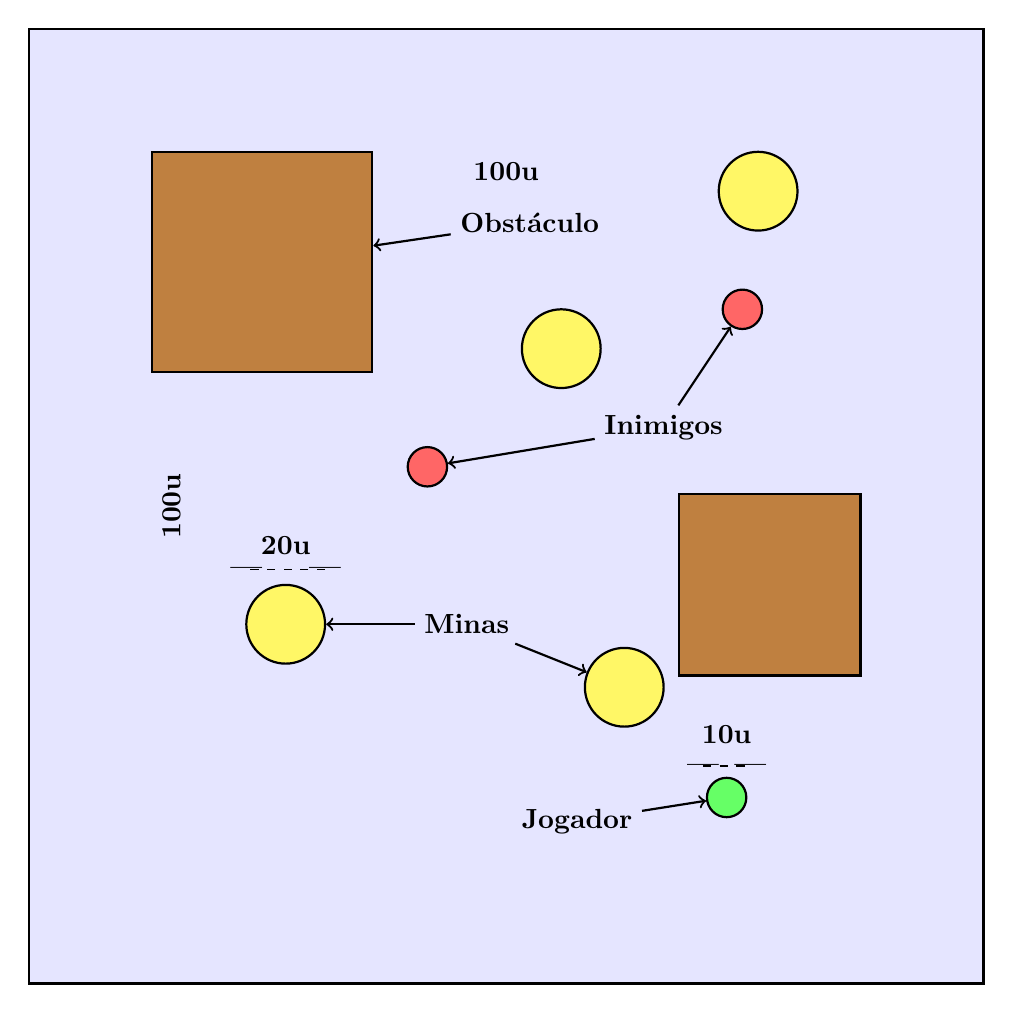
\begin{tikzpicture}[]
	\tikzstyle{sub}=[thick, draw, circle, align=center, minimum size = 0.5cm]					
	\tikzstyle{mine}=[thick, draw, circle, align=center, minimum size = 1cm, fill=yellow!60!white]					
	\tikzstyle{obstacle}=[thick, draw, rectangle, align=center, fill=brown]					
	\node[align=center, fill=blue!10!white, thick, draw, thick, rectangle, minimum height=\columnwidth, minimum width=\columnwidth](tarea)at (0,0) {};
	\node[](a1)at (0, 4.25) {\bf 100u};
	\node[rotate=90](a1)at (-4.25, 0) {\bf 100u};
	
	\node[obstacle, minimum size=2.8cm](obs1)at (-3.1, 3.1) {};
	\node[obstacle, minimum size=2.3cm](obs2)at (3.35, -1) {};
	\node[](tobs)at (0.3, 3.6) {\bf Obstáculo};
	\draw[->, thick](tobs) -- (obs1);

	\node[fill=green!60!white, sub](player)at (2.8, -3.7) {};	
	\node[](tplayer)at (0.9, -4) {\bf Jogador};
	\draw[->, thick](tplayer) -- (player);
	\node[](a1)at (3.1, -3.3) {\bf |};
	\node[](a2)at (2.5, -3.3) {\bf |};
	\draw[-, dashed](2.5, -3.3) -- (3.1, -3.3);
	\node[](a2)at (2.8, -2.9) {\bf10u};
	
	\node[fill=red!60!white, sub](enemy1)at (-1, 0.5) {};	
	\node[fill=red!60!white, sub](enemy2)at (3, 2.5) {};
	\node[](tenemy)at (2, 1) {\bf Inimigos};
	\draw[->, thick](tenemy) -- (enemy1);
	\draw[->, thick](tenemy) -- (enemy2);
	
	\node[mine](mine1)at (-2.8, -1.5) {};	
	\node[mine](mine2)at (1.5, -2.3) {};
	\node[mine](mine3)at (0.7, 2) {};
	\node[mine](mine4)at (3.2, 4) {};
	\node[](tmines)at (-0.5, -1.5) {\bf Minas};
	\draw[->, thick](tmines) -- (mine1);
	\draw[->, thick](tmines) -- (mine2);
	
	\node[](a1)at (-3.3, -0.8) {\bf |};
	\node[](a2)at (-2.3, -0.8) {\bf |};
	\draw[-, dashed](-2.3, -0.8) -- (-3.3, -0.8);
	\node[](a2)at (-2.8, -0.5) {\bf20u};	
	\end{tikzpicture}
\end{figure}
%
\vfill
%
No início do jogo, espalhe os submarinos do inimigo e dos jogadores, assim como possíveis obstáculos no mapa.
Além disso, determine a posição das minas, mas as mantenha em segredo até que sejam ativadas ou detectadas pelo sonar.
Antes de iniciar o jogo, os jogadores podem escolher um dos 3 níveis de dificuldade, que determinam a quantidade de minas e submarinos inimigos, assim como o prêmio recebido em caso de vitória.
%
\\\\
%
\oftable{p{0.2\columnwidth} p{0.35\columnwidth} p{0.4\columnwidth}}
{\accf{Dificuldade} & \accf{Inimgos / Minas} & \accf{Prêmio}}
{
	Fácil 	& 1 / 2 & Matéria negra\ofrow
	Médio	& 2 / 4 & Materia esfregão \ofrow
	Difícil 	& 3 / 6 & Grampo dourado \ofrow
}
%
\clearpage
%
%
%
%
%
%
%
%
%
\includegraphics[width=\columnwidth]{./art/goldsaucer/chocoborace.jpg}
%
\vfill
%
\accf{Corrida de chocobo} é um jogo de corrida cuja entrada custa 2 Gp por jogador. 
Cada jogador é um jóquei na corrida e podem escolher uma das seguintes Chocobos fornecidas pelo parque ou usar alguma própria.
O MJ adiciona e joga com os participantes restantes na corrida até que haja 5 competidores no total.
%
\\\\
%
\oftable{p{0.35\columnwidth} p{0.3\columnwidth} p{0.3\columnwidth}}
{\accf{Chocobo} & \accf{Fôlego} & \accf{Agilidade}}
{
	Eco 	& 4 & 5 \ofrow
	Cinco 	& 5 & 4 \ofrow
	Rex 	& 6 & 3 \ofrow
	Cody 	& 7 & 2 \ofrow
	Jesse   & 8 & 1 
}
%
\vfill
%
Uma corrida consiste em várias rodadas e durante cada uma delas, cada participante realiza um teste de arrancada para determinar a distância percorrida.
Eles somarão continuamente os resultados de seus testes à pontuação final, o primeiro a superar 50 pontos vence.
A pontuação de cada um deles deve ser anunciada ao final de cada rodada e registrada.
Se mais de um participante alcançar a linha de chegada na mesma rodada, aquele com a maior pontuação vence.
O teste de arrancada realizado a cada turno é modificado da seguinte maneira: \ofrow
%
\ofbullet{%
	O resultado de cada arrancada é reduzido pela diferença entre o Fôlego da Chocobo e sua fadiga atual.
	Todos começam com 0 de fadiga e ganham 1 ponto ao final de cada rodada.
	Por exemplo, se uma Chocobo tem fadiga 10 e Fôlego 8, o resultado do teste será reduzido em 2, mas se ela tivesse 10 ou mais de Fôlego, não receberia penalidade alguma.
	Esta redução não pode fazer com que a arrancada caia abaixo de 0.
}
\ofbullet{%
	Antes de cada teste, um participante pode decidir realizar uma ação de disparada.
	Neste caso, ele ganha Vantagem no teste de arrancada, mas também, um ponto de fadiga extra.
	Na corrida, você pode disparar somente uma quantidade de vezes igual à Agilidade da Chocobo.
}
\ofbullet{%
	Os personagens que são particularmente bons em lidar com Chocobos têm Vantagem nos testes de arrancada.
}
%
\\\\
%
Quando a corrida termina, o vencedor rola 1d e recebe o prêmio baseado no resultado.
%
\newpage
%
\oftable{p{0.4\columnwidth} p{0.7\columnwidth}}
{\accf{Resultado} & \accf{Prêmio}}
{
	1 & 10 GP \ofrow
	2 & Pena de Fênix \ofrow
	3 & Matéria de aviso \ofrow
	4 & Elixir \ofrow
	5 & Matéria debandada \ofrow
	6 & Sandália alada
}
%
\\\\
%
%
%
%
%
%
%
%
%
\begin{center} \includegraphics[width=\columnwidth]{./art/goldsaucer/snowgame.jpg} \end{center}
\accf{Jogo de Neve} é um jogo de snowboard que custa 1 GP por jogador. 
Ele funciona com vários jogadores que correm abaixo numa pista de ski tentando alcançar a maior pontuação.
Ela começa em 0, coletar balões a aumenta, enquanto esbarrar em obstáculos, a reduz, por isso a pontuação pode ser negativa.
O jogo tem até 7 rodadas e no começo de cada uma delas, o MJ rola 3d, um dado após o outro, a fim de determinar os objetos nas 3 pistas em frente aos jogadores da esquerda à direita.
A tabela abaixo mostra os possíveis objetos baseados no resultado do dado e seus efeitos, ao se colidirem com eles.
%
\\\\
%
\oftable{p{0.3\columnwidth} p{0.35\columnwidth} p{0.3\columnwidth}}
{\accf{Resultado} & \accf{Objeto} & \accf{Efeito}}
{
	1 - 2 & Nada & -- \ofrow
	3 & Boneco de neve & - 1 ponto \ofrow
	4 & Rocha & - 2 pontos  \ofrow
	5 & Balões vermelhos & + 1 pontos \ofrow
	6 & Balões azuis & + 2 pontos  \ofrow
}
%
\\\\
%\clearpage
%
Depois de aprender sobre os objetos em frente a eles, cada jogador pode decidir entre 1 de 3 ações:\ofrow
\ofbullet{\accf{Mova-se à pista da esquerda ou à da direita:} faça um teste de DF~6, se for bem sucedido, mude uma pista, do contrário, fique na atual.} 
\ofbullet{\accf{Mova das pistas à esquerda ou àdireita:} faça um teste de DF~8, se for bem sucedido, mude duas pistas, do contrário fique na atual.} 
\ofbullet{\accf{Saltar:} faça um teste de DF~8, se bem sucedido, evite o obstáculo a sua frente e ganhe 1 ponto. Se falhar, colida com ele e perca 1 ponto. Você pode usar essa ação mesmo se não haver objetos a frente.} \ofrow
Os personagens que são particularmente bons em coordenação ou têm experiência com snowboards, têm  Vantagem nesses testes. 
Após todas as ações serem realizadas, avalie em quais pistas que cada jogador terminou e com quais objetos colidiram, ou não, para anotar a pontuação antes do inicio da próxima rodada.
Ao fim da 7º rodada, todos os jogadores alcançam a linha de chegada a depender de sua pontuação, cada um deles recebem um dos seguintes prêmios.
%
\\\\
%
\oftable{p{0.4\columnwidth} p{0.7\columnwidth}}
{\accf{Ponruação} & \accf{Prêmio}}
{
	< 3 & Medalha de participação \ofrow
	3 - 4 & Super poção \ofrow
	5 - 6 & Pin de segurança \ofrow
	7 - 8 & PV+ \ofrow
	> 8 & 50 GP \ofrow
}
%
%
\ofpar\\\\
%
%
%
%
%
%
\includegraphics[width=\columnwidth]{./art/goldsaucer/gbike.jpg}
\\\\
\accf{Moto-G} é um jogo de moto em que os jogadores são perseguidos por motociclistas hostis numa auto estrada e têm que lutar para conseguir escapar. 
O jogo pode ser jogado por vários jogadores pelo custo de 1 GP por jogador.
A auto estrada tem 4 pistas e o foco é sempre colocar 3 filas, assim haverá 12 posições no total, onde motociclistas e obstáculos podem ser colocados no momento certo.
A ilustração abaixo mostra como o mapa pode se parecer durante o jogo.
%
%\newpage
%
\begin{figure}[h!]
	\centering
	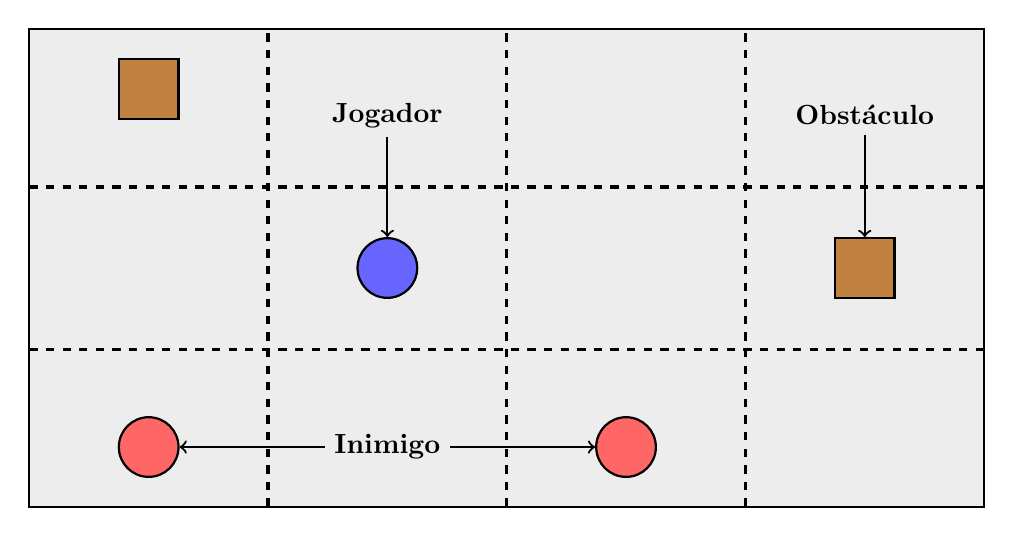
\begin{tikzpicture}[]
	\tikzstyle{biker}=[thick, draw, circle, align=center, minimum size = 0.5*0.125\columnwidth]					
	\tikzstyle{obstacle}=[thick, draw, rectangle, align=center, fill=brown, minimum size=0.5*0.125\columnwidth]					
	
	\node[align=center, thick, draw, thick, rectangle, minimum height=0.5\columnwidth, minimum width=\columnwidth, fill=black!7!white](tarea)at (0,0) {};		
	\draw[very thick, -, dashed](-0.25\columnwidth, -0.25\columnwidth) -- (-0.25\columnwidth, 0.25\columnwidth);
	\draw[very thick, -, dashed](0, -0.25\columnwidth) -- (0, 0.25\columnwidth);
	\draw[very thick, -, dashed](0.25\columnwidth, -0.25\columnwidth) -- (0.25\columnwidth, 0.25\columnwidth);
	\draw[very thick, -, dashed](-0.5\columnwidth, 0.5*-0.17\columnwidth) -- (0.5\columnwidth, 0.5*-0.17\columnwidth);
	\draw[very thick, -, dashed](-0.5\columnwidth, 0.5*0.17\columnwidth) -- (0.5\columnwidth, 0.5*0.17\columnwidth);
	
	\node[fill=red!60!white, biker](b1)at (-0.375\columnwidth, 0.5*-0.375\columnwidth) {};
	\node[fill=red!60!white, biker](b2)at (0.125\columnwidth, 0.5*-0.375\columnwidth) {};
	\node[fill=blue!60!white, biker](b3)at (-0.125\columnwidth, 0) {};
	\node[obstacle](obs1)at (0.375\columnwidth, 0) {};
	\node[obstacle](obs2)at (-0.375\columnwidth, 0.5*0.375\columnwidth) {};
	
	\node[](tobs)at (0.375\columnwidth, 0.16\columnwidth) {\bf Obstáculo};
	\draw[->, thick](tobs) -- (obs1);
	\node[](tplayer)at (-0.125\columnwidth, 0.16\columnwidth) {\bf Jogador};
	\draw[->, thick](tplayer) -- (b3);
	\node[](tenemy)at (-0.125\columnwidth, 0.5*-0.375\columnwidth) {\bf Inimigo};
	\draw[->, thick](tenemy) -- (b1);
	\draw[->, thick](tenemy) -- (b2);
	\end{tikzpicture}
\end{figure}
%
\newpage
%
O jogo funciona em 7 rodadas e durante cada uma delas, em primeiro lugar, todos os jogadores agem e então os motociclistas hostis.
Os jogadores começam com 3 PV e os inimigos com 1 PV, ao ser reduzido a 0 PV, o motociclista é removido do jogo.
Durante um turno, cada um pode fazer um movimento e realizar um ataque:
\vfill
\ofbullet{\accf{Movimento:} mova-se a uma pista à esquera / direita ou uma fila à frente / trás. se a posição não estiver ocupada por um obstáculo ou outro motociclista. Também é possível ativar o turbo da moto. Neste caso, faça um teste de DF~8, se for bem suceiddo, você pode realizar dois movimentos nesse turno, se falhar, não pode se mover. Os personagens que sejam particularmente bons em dirigir veículos recebem Vantagem neste teste}\ofpar
\ofbullet{\accf{Ataque físico:} faça um teste de DF~6, se bem sucedido, um moticiclista que estiver a 1 movimento de distância, sofre 1 ponto de PV.}\ofpar
\ofbullet{\accf{Ataque â distância:} faça um teste de DF~8, se bem sucedido, um motociclista que esteja a 2 ou menos movimentos de distância, sofre 1 PV de dano.}
%
\vfill
%
No início de cada rodada, role 1d para cada jogador que ainda estiver no jogo.
Baseado no resultado, ponha os seguintes itens em qualquer posição aberta à sua escolha: 1-2: nada, 3: motociclista vermelho, 4: motoqueiro azul, 5-6: obstáculo.
No entanto, não ponha qualquer motoqueiro hostil se já houver a mesma quantidade deles que a de jogadores.
Os motoqueiros vermelhos e azuis são controlados pelo MJ e seguem as mesmas regras que os jogadores, mas os vermelhos só podem realizar ataques à distância enquanto os azuis, somente ataques físicos.
Todos os obstáculos seguem as mesmas regras e o MJ é livre para escolher a aparência deles, podendo ser bloqueios ou veículos.
Sempre que um jogador terminar seu turno com um obstáculo na mesma pista em frente a ele, ele tem que fazer um teste de DF~6, se bem sucedido, ele salta o obstáculo, mas se falhar, sofre 1 PV de dano.
Motoqueiros inimigos esquivam de todos eles automaticamente. No fim de cada rodada, todos os motoqueiros ficam em suas posições e todos os obstáculos desaparecem, enquanto são deixados para trás do campo de visão.
Cada jogador que sobreviver até o fim da 7º rodada, ganha o prêmio.
Cada vencedor rola 1d e dependendo do resultado, recebe um dos seguintes prêmios.
%
\vfill
%
\oftable{p{0.4\columnwidth} p{0.5\columnwidth}}
{\accf{Resulto} & \accf{Prêmio}}
{
	1 	 & Suporte de item \ofrow
	2    & 5 GP \ofrow		
	3    & Super Éter \ofrow
	4    & Pena de Fênix \ofrow
	5    & Matéria alerta \ofrow    
	6    & Matéria bomba
}
%
\clearpage
%
%
%
%
%
%\includegraphics[width=\columnwidth]{./art/goldsaucer/proxycatcher.jpg}
%%
%\vfill
%%
%\accf{Proxy Catcher} is a crane game that costs 4 GP to play.
%The game is played by a single player who uses the controls of the machine to navigate a crane and potentially pick a valuable prize from a pile.
%The player only has one chance to lower the crane and grab something.
%To do so, the player makes a check and receives a prize based on the result as listed in the table below.
%However, the game is rigged as the crane has a fixed chance of properly grabbing something.
%Players can perform a DC~8 check to understand that the player skill has barely any influence on the odds of success.
%%
%\vfill
%%
%\oftable{p{0.5\columnwidth} p{0.5\columnwidth}}
%{\accf{Result} & \accf{Prize}}
%{
%	2 - 5 & Nothing \ofrow
%	6 - 7 & Potion \ofrow
%	8     & 5 GP \ofrow		
%	9     & Ether \ofrow
%	10    & Phoenix Down \ofrow
%	11    & 20 GP \ofrow    
%	12    & Counter Materia
%}
%\vfill
%%
%{
%\begin{center}\includegraphics[width=0.7\columnwidth]{./art/goldsaucer/caitsith.jpg}\end{center}
%%
%%
%%
%%
%\newpage
%%
%\includegraphics[width=\columnwidth]{./art/goldsaucer/arena.jpg}
%%
%\vfill
%%
%The \accf{Colosseum} is a battle arena that costs 1 GP per player to participate in.
%All players that want to participate, fight up to 7 groups of monsters together as a party, one after another, on a 10u by 10u battlefield with walls on all 4 sides.
%After the party defeats one group, roll 1d and depending on the result, they receive an additional handicap in each subsequent fight.
%If you roll the same number twice, roll again until you get a handicap that is not active yet.
%The list below shows the 6 possible handicaps, so by time the party reaches the 7th round, all of them will be active.
%%
%\vfill
%%
%\oftable{p{0.15\columnwidth} p{0.75\columnwidth}}
%{\accf{Result} & \accf{Handicap}}
%{
%	1 & You can no longer equip Materia. \ofrow
%	2 & You can no longer use Items.  \ofrow
%	3 & You can no longer equip Accessories. \ofrow
%	4 & You can no longer equip Armor.  \ofrow
%	5 & You can no longer use Limit Breaks. \ofrow
%	6 & You suffer Zombie until you leave the Colosseum (cannot be removed). \ofrow
%}
%%
%\vfill
%%
%After defeating a group, everyone in the party can take an additional turn before the next fight starts.
%At that point, they can also decide to forfeit and collect a prize depending on how many rounds they have completed.
%If the entire party is defeated within a round, they do not receive any prize.
%In any case, the party fully recovers their HP and MP after leaving the Colosseum.  
%The list below shows the possible prizes depending on how many rounds were completed.
%The following page shows the 7 types of monsters encountered from the 1st to the 7th round.
%At the start of each round, place as many of the current round's monster type on the battlefield as there are players.
%%
%\vfill
%%
%\oftable{p{0.4\columnwidth} p{0.75\columnwidth}}
%{\accf{Round} & \accf{Prize}}
%{
%	1 & Potion \ofrow
%	2 & Phoenix Down \ofrow
%	3 & 10 GP \ofrow
%	4 & Lure Materia  \ofrow
%	5 & Rewind Materia \ofrow
%	6 & Protect Bangle \ofrow
%	7 & Genji Gloves \ofrow
%}
%%
%\clearpage
%%
%\ofmonster{Python (Round 1)}{3}{\includegraphics[width=0.2\columnwidth]{./art/goldsaucer/python.jpg}}
%{
%	HP: & \hfill 24 & MP: & \hfill 18\\
%	STR: & \hfill 3 & DEF: & \hfill 1 \\
%	MAG: & \hfill 0 & RES: & \hfill 3 \\
%	AGI: & \hfill 3 & Size: & \hfill M\\
%}
%{\accf{Bite}: 1d DMG \hfill \accf{Immune:}\poison \hfill \accf{Weak:}\earth}
%{	
%	\mtech{Entangle}{6}{0r}{Single}{3u}{The target makes a DC 8 check and suffers 2d damage and Immobile for 1 round upon failure.}{\immobile}		
%}
%%
%\vfill
%%
%\ofmonster{Hecteyes (Round 2)}{4}{\includegraphics[width=0.2\columnwidth]{./art/goldsaucer/hecteyes.jpg}}
%{
%	HP: & \hfill 32 & MP: & \hfill 50\\
%	STR: & \hfill 1 & DEF: & \hfill 2 \\
%	MAG: & \hfill 6 & RES: & \hfill 8 \\
%	AGI: & \hfill 2 & Size: & \hfill M\\
%}
%{\accf{Tackle}: 2d DMG \hfill \accf{Immune:}\sleep \hfill \accf{Weak:}\lightning}
%{	
%	\mspell{Blind}{6}{1r}{Single}{3u}{The target makes a DC 8 check and suffers Blind for 3 round upon failure.}{\blind}		
%	\mspell{Thunder}{4}{1r}{Single}{3u}{You deal 2d lightning damage to the target.}{\ice}		
%}
%%
%\vfill
%%
%\ofmonster{Mantis (Round 3)}{5}{\includegraphics[width=0.23\columnwidth]{./art/goldsaucer/mantis.jpg}}
%{
%	HP: & \hfill 46 & MP: & \hfill 30\\
%	STR: & \hfill 4 & DEF: & \hfill 2 \\
%	MAG: & \hfill 0 & RES: & \hfill 2 \\
%	AGI: & \hfill 3 & Size: & \hfill M\\
%}
%{\accf{Cut}: 2d DMG \hfill \accf{Immune:}\immobile \hfill \accf{Weak:}\fire}
%{	
%	\mtech{Metal Cutter}{4}{0r}{Single}{Weapon}{Make an Attack against the target. If you succeed, the damage dealt ignores the target's DEF.}{}		
%	\mpassive{Leap}{When moving you can jump over enemies and obstacles up to a height of 2u, instead of having to walk around them.}	
%}
%%
%\vfill
%%
%\ofmonster{Griffon (Round 4)}{6}{\includegraphics[width=0.23\columnwidth]{./art/goldsaucer/griffon.jpg}}
%{
%	HP: & \hfill 67 & MP: & \hfill 50\\
%	STR: & \hfill 6 & DEF: & \hfill 3 \\
%	MAG: & \hfill 0 & RES: & \hfill 5 \\
%	AGI: & \hfill 3 & Size: & \hfill M\\
%}
%{\accf{Claw}: 2d DMG \hfill \accf{Immune:}\immobile\blind \hfill \accf{Resilient:}\wind}
%{	
%	\mtech{Feather Shot}{6}{0r}{Single}{4u}{The target suffers 3d wind damage.}{\wind}		
%	\mpassive{Peck}{Whenever you successfully Attack a target he makes a DC 7 check and suffers Blind for 3 rounds upon failure.}
%}
%%
%\newpage
%%
%\ofmonster{Big Horn (Round 5)}{7}{\includegraphics[width=0.23\columnwidth]{./art/goldsaucer/bighorn.jpg}}
%{
%	HP: & \hfill 90 & MP: & \hfill 80\\
%	STR: & \hfill 7 & DEF: & \hfill 5 \\
%	MAG: & \hfill 0 & RES: & \hfill 5 \\
%	AGI: & \hfill 2 & Size: & \hfill L\\
%}
%{\accf{Tackle}: 3d DMG \hfill \accf{Immune:}\poison \hfill \accf{Resilient:}\fire}
%{	
%	\mtech{Charge}{8}{1r}{Single}{10u}{Dash towards the target and deal 3d damage to him. In addition, the target is knocked back by 3u and if he hits a wall, he suffers an additional 3d damage.}{}		
%	\mreaction{Kickback}{Whenever you suffer damage from an enemy within 1u, you can deal 10 physical damage to him and knock him back by 2u.}
%}
%%
%\vfill
%%
%\ofmonster{Golem (Round 6)}{8}{\includegraphics[width=0.23\columnwidth]{./art/goldsaucer/golem.jpg}}
%{
%	HP: & \hfill 130 & MP: & \hfill 100\\
%	STR: & \hfill 9 & DEF: & \hfill 8 \\
%	MAG: & \hfill 0 & RES: & \hfill 6 \\
%	AGI: & \hfill 2 & Size: & \hfill L\\
%}
%{\accf{Fist}: 3d DMG \hfill \accf{Immune:}\poison\sleep\ \hfill \accf{Resilient:}\earth}
%{	
%	\mspell{Quake}{20}{1r}{3u}{7u}{Deal 6d earth damage to everyone in the target area.}{\earth}
%	\mtech{Earth Wall}{12}{0r}{3u (line)}{3u}{You create a 3u tall and wide wall of earth that blocks the path. The wall breaks down after 3 rounds or upon suffering a total of 15 damage.}{}
%}
%%
%\vfill
%%
%\ofmonster{Dark Dragon (Rnd 7)}{9}{\includegraphics[width=0.24\columnwidth]{./art/goldsaucer/blackdragon.jpg}}
%{
%	HP: & \hfill 200 & MP: & \hfill 180 \\
%	STR: & \hfill 10 & DEF: & \hfill 7 \\
%	MAG: & \hfill 9 & RES: & \hfill 8 \\
%	AGI: & \hfill 3 & Size: & \hfill L\\
%}
%{\accf{Bite}: 3d DMG \hfill \accf{Resilient}:\fire\ice\dark \\ \accf{Immune}: All Status Effects}
%{
%	\mtech{Obliterating Breath}{16}{0r}{3u (front)}{3u}{Everyone in the target area makes a DC 8 check and suffers 4d damage as well as Poison and Blind for 3 rounds upon failure.}{\poison \blind}{}
%	\mspell{Dark Flare}{30}{2r}{Single}{5u}{You deal 6d+20 dark damage to the target.}{\dark}
%	\mpassive{Tail Whip}{Whenever you Attack, you can choose to target all enemies within 1u at once.}	
%}	
%
%\clearpage